\documentclass[12pt,a4paper]{article}
\usepackage[margin=1in,headheight=15pt]{geometry}
\usepackage{amsmath,amssymb}
\usepackage{booktabs}
\usepackage{listings}
\usepackage{xcolor}
\usepackage{hyperref}
\usepackage{xurl}
\usepackage{longtable}
\usepackage{caption}
\usepackage{enumitem}
\usepackage{fancyhdr}
\usepackage{graphicx}
\usepackage{tikz}
\usepackage{pgfplots}
\usepackage{setspace}
\usepackage{titlesec}
\usepackage{tocbibind}

\usetikzlibrary{arrows.meta,positioning,shapes.geometric,calc,decorations.pathreplacing,matrix}
\pgfplotsset{compat=1.18}
\hypersetup{colorlinks=true, linkcolor=blue, urlcolor=blue, citecolor=black}

\definecolor{codebg}{rgb}{0.96,0.96,0.96}
\definecolor{keywordcolor}{rgb}{0.0,0.0,0.6}
\definecolor{commentcolor}{rgb}{0.35,0.35,0.35}

\lstset{
    backgroundcolor=\color{codebg},
    basicstyle=\ttfamily\footnotesize,
    breaklines=true,
    frame=single,
    columns=fullflexible,
    keywordstyle=\color{keywordcolor}\bfseries,
    commentstyle=\color{commentcolor}\itshape,
    language=C,
    showstringspaces=false,
    numbers=left,
    numberstyle=\tiny\color{gray}
}

\pagestyle{fancy}
\fancyhf{}
\rhead{Sampad De — 002410501025}
\lhead{Computer Networks Lab: Assignment 1}
\rfoot{Page \thepage}

\onehalfspacing

\begin{document}

% ==================== TITLE PAGE ====================
\begin{titlepage}
    \centering
    \vspace*{1.5cm}
    
    {\small JADAVPUR UNIVERSITY \par}
    \vspace{0.8cm}
    {\small DEPARTMENT OF COMPUTER SCIENCE AND ENGINEERING\par}
    \vspace{1.2cm}
    
    \rule{\textwidth}{1.2pt}\par
    \vspace{0.4cm}
    {\huge\bfseries Assignment 1 Report -- Comprehensive Evaluation of Error Detection Schemes in Network Transmission \par}
    \vspace{0.3cm}
    {\Large\itshape Comparative Reliability, Boundary Failures, and Overhead of 16-Bit Internet Checksum and Cyclic Redundancy Checks (CRC-8, 10, 16, 32) \par}
    \vspace{0.4cm}
    \rule{\textwidth}{1.2pt}\par
    
    \vspace{1.5cm}
    
    \begin{flushleft} \large
        \textbf{Course:} Computer Networks Laboratory (BCSE-III) \\
        \textbf{Student Name:} Sampad De \\
        \textbf{Roll Number:} 002410501025 \\
        \textbf{Assignment:} Assignment 1 (Error Detection) \\
        \textbf{Date of Submission:} August 19, 2026
    \end{flushleft}
    
    \vfill
    
    {\large Kolkata, West Bengal, India \par}
\end{titlepage}

\newpage
\tableofcontents
\newpage

\section*{System Configuration and Environment}
This project was developed and evaluated using the following environment:
\begin{table}[htbp]
\centering
\small
\resizebox{0.75\linewidth}{!}{
\begin{tabular}{ll}
\toprule
\textbf{Component} & \textbf{Specification} \\
\midrule
Operating System & macOS \\
Networking & BSD Sockets (UDP) \\
Compiler & Apple Clang (\texttt{clang}) \\
Profiling Timer & POSIX \texttt{clock\_gettime(CLOCK\_MONOTONIC)} \\
\bottomrule
\end{tabular}
}
\end{table}



% ==================== SECTION 1 ====================
\section{Introduction and Objectives}

Data transmitted across any physical communications medium is subject to corruption caused by thermal noise, electrical interference, line attenuation, and clock synchronization drift. In computer network protocol stacks, ensuring that received bits match transmitted bits is divided between the Data Link Layer and Transport Layer. 

For this assignment, I designed and implemented a modular network simulation environment in C. The goals of my project are:
\begin{enumerate}[leftmargin=*]
    \item \textbf{Protocol Implementation:} Implement the standard 16-bit Internet Checksum (RFC 1071) and four variations of Cyclic Redundancy Checks (CRC-8, CRC-10, CRC-16, and CRC-32) from scratch.
    \item \textbf{Client-Server Architecture:} Construct a socket-based sender and receiver application running over UDP to transmit framed text payloads across a network interface.
    \item \textbf{Deterministic and Statistical Error Injection:} Develop an error-injection engine capable of inserting single-bit flips, isolated double-bit flips, odd-parity bit flips, and uniformly distributed burst errors of varying lengths.
    \item \textbf{Empirical and Theoretical Validation:} Run a large-scale offline benchmarking suite (1,000,000 simulated frame transmissions) to measure exact detection rates, identify edge-case collisions, and quantify computational throughput on macOS.
\end{enumerate}

% ==================== SECTION 2 ====================
\section{Theoretical Principles of Error Detection}

\subsection{The 16-Bit Internet Checksum (One's Complement Sum)}
The Internet Checksum is an arithmetic error-detection algorithm used in IPv4, TCP, and UDP headers. The algorithm treats the input byte stream as a sequence of 16-bit unsigned integers. 

The arithmetic uses \textbf{one's complement addition}. In standard two's complement computer hardware, when the sum of two 16-bit integers produces a carry out of the 16th bit (bit 15), this overflow bit represents $2^{16} \equiv 1 \pmod{2^{16}-1}$. Therefore, an \textbf{end-around carry} is performed: the carry bit is added back into the least significant bit of the sum. Finally, the total sum is bitwise inverted (one's complemented).

\begin{equation}
    \text{Checksum} = \sim \left( \sum_{i=1}^{k} W_i \pmod{2^{16}-1} \right)
\end{equation}

\subsubsection{Theoretical Vulnerabilities of the Checksum}
While simple to compute in software and hardware, the checksum has well-known structural weaknesses:
\begin{itemize}[leftmargin=*]
    \item \textbf{Compensating Errors:} If an error in word $W_a$ increments its value by $+K$ and another error in word $W_b$ decrements its value by $-K$, the total sum remains completely identical. 
    \item \textbf{Byte Order Invariance:} Swapping two 16-bit words or rearranging whole aligned blocks produces the exact same sum.
    \item \textbf{Zero Preservation:} A block of all-zero words sums to zero and does not change the checksum.
\end{itemize}

\subsection{Cyclic Redundancy Check (CRC) and Modulo-2 Arithmetic}
Cyclic Redundancy Checks treat binary bit strings as coefficients of polynomials using modulo-2 arithmetic. In modulo-2 binary arithmetic, addition and subtraction are equivalent and correspond directly to the bitwise Exclusive-OR (XOR) operation without carries or borrows.

Given an $m$-bit message polynomial $M(x)$ and an $(r+1)$-bit generator polynomial $G(x)$ of degree $r$:
\begin{enumerate}[leftmargin=*]
    \item The message is multiplied by $x^r$, effectively appending $r$ zero bits: $x^r M(x)$.
    \item I performed modulo-2 polynomial division of $x^r M(x)$ by $G(x)$ to obtain a quotient $Q(x)$ and an $r$-bit remainder $R(x)$:
    \begin{equation}
        x^r M(x) = Q(x) G(x) \oplus R(x)
    \end{equation}
    \item The transmitted frame polynomial $T(x)$ is formed by appending the remainder $R(x)$ to the message:
    \begin{equation}
        T(x) = x^r M(x) \oplus R(x) = Q(x) G(x)
    \end{equation}
    Since $R(x) \oplus R(x) = 0$ in modulo-2 arithmetic, $T(x)$ is an exact multiple of $G(x)$.
\end{enumerate}

When the receiver gets a potentially corrupted frame $T'(x) = T(x) \oplus E(x)$, where $E(x)$ is the error polynomial, it computes the remainder of $T'(x) / G(x)$:
\begin{equation}
    \frac{T'(x)}{G(x)} = \frac{T(x) \oplus E(x)}{G(x)} = Q(x) \oplus \frac{E(x)}{G(x)}
\end{equation}
An error is undetected \textbf{if and only if} the error polynomial $E(x)$ is evenly divisible by $G(x)$.

\subsubsection{Mathematical Guarantees of CRC Polynomials}
\begin{itemize}[leftmargin=*]
    \item \textbf{Single-Bit Errors ($E(x) = x^i$):} If $G(x)$ has at least two non-zero terms (e.g., $x^r$ and $x^0 = 1$), it cannot divide $x^i$. Detection rate is strictly $100\%$.
    \item \textbf{Double-Bit Errors ($E(x) = x^i + x^j = x^j(x^{i-j} + 1)$):} As long as $G(x)$ does not divide $x^k + 1$ for any $k < \text{frame length}$, double bit errors are caught with $100\%$ reliability.
    \item \textbf{Odd Number of Errors:} If $(x+1)$ is a factor of $G(x)$, any polynomial with an odd number of terms cannot be divided by $(x+1)$ because $E(1) = 1 \neq 0$. Thus, $100\%$ of all odd-weight bit errors are caught.
    \item \textbf{Burst Errors of Length $L \le r$:} An error burst of length $L$ starting at position $i$ is $E(x) = x^i B(x)$, where $\deg(B(x)) = L - 1 < r$. Since $\deg(B(x)) < \deg(G(x))$, $G(x)$ cannot divide $E(x)$. Detection rate is strictly $100\%$.
    \item \textbf{Burst Errors of Length $L = r + 1$:} The fraction of missed bursts is exactly $(1/2)^{r-1}$.
    \item \textbf{Burst Errors of Length $L > r + 1$:} The fraction of missed bursts bounds to $(1/2)^r$.
\end{itemize}

% ==================== SECTION 3 ====================
\section{System Architecture and Implementation}

\subsection{Frame Structure and In-Memory Layout}
To simulate an Ethernet-like data-link frame, I defined a structured packet containing a 14-byte MAC header, a 44-byte data payload, and a 4-byte trailer.

\begin{figure}[htbp]
\centering
\resizebox{\linewidth}{!}{
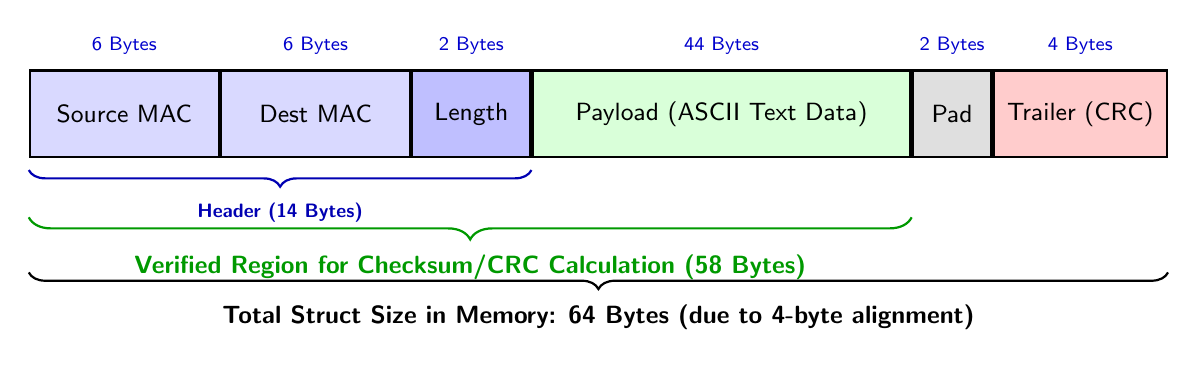
\begin{tikzpicture}[
    cell/.style={rectangle, draw=black, thick, minimum height=1.1cm, text centered, font=\sffamily\small},
    field/.style={font=\sffamily\footnotesize},
    dim/.style={font=\sffamily\scriptsize, text=blue!80!black}
]
    % Header fields
    \node[cell, fill=blue!15, minimum width=2.4cm] (src) at (0,0) {Source MAC};
    \node[cell, fill=blue!15, minimum width=2.4cm, right=0cm of src] (dst) {Dest MAC};
    \node[cell, fill=blue!25, minimum width=1.5cm, right=0cm of dst] (len) {Length};
    
    % Payload
    \node[cell, fill=green!15, minimum width=4.8cm, right=0cm of len] (pay) {Payload (ASCII Text Data)};
    
    % Padding and Trailer
    \node[cell, fill=gray!25, minimum width=1.0cm, right=0cm of pay] (pad) {Pad};
    \node[cell, fill=red!20, minimum width=2.2cm, right=0cm of pad] (tra) {Trailer (CRC)};
    
    % Byte indicators top
    \node[dim, above=2pt of src] {6 Bytes};
    \node[dim, above=2pt of dst] {6 Bytes};
    \node[dim, above=2pt of len] {2 Bytes};
    \node[dim, above=2pt of pay] {44 Bytes};
    \node[dim, above=2pt of pad] {2 Bytes};
    \node[dim, above=2pt of tra] {4 Bytes};
    
    % Brackets bottom
    \draw[decorate, decoration={brace, mirror, amplitude=6pt}, thick, color=blue!70!black] 
        ($(src.south west)+(0,-0.15)$) -- ($(len.south east)+(0,-0.15)$) 
        node[midway, below=8pt, font=\sffamily\scriptsize\bfseries] {Header (14 Bytes)};
        
    \draw[decorate, decoration={brace, mirror, amplitude=8pt}, thick, color=green!60!black] 
        ($(src.south west)+(0,-0.75)$) -- ($(pay.south east)+(0,-0.75)$) 
        node[midway, below=10pt, font=\sffamily\small\bfseries] {Verified Region for Checksum/CRC Calculation (58 Bytes)};
        
    \draw[decorate, decoration={brace, mirror, amplitude=6pt}, thick, color=black] 
        ($(src.south west)+(0,-1.45)$) -- ($(tra.south east)+(0,-1.45)$) 
        node[midway, below=8pt, font=\sffamily\small\bfseries] {Total Struct Size in Memory: 64 Bytes (due to 4-byte alignment)};
\end{tikzpicture}
}
\caption{In-memory layout of the custom transmission frame, highlighting verified bytes versus trailer alignment.}
\label{fig:framelayout}
\end{figure}

The C struct definition from \texttt{headers/info.h} is shown below:
\begin{lstlisting}[caption={Frame Definition (\texttt{info.h})}]
#define PAYLOAD_SIZE 44

typedef struct frame_header {
    unsigned char SOURCE_MAC[6];
    unsigned char DEST_MAC[6];
    uint16_t      length;
} frame_header;                      // 14 bytes

typedef struct frame_trailer {
    uint32_t crc_send;
} frame_trailer;                     // 4 bytes

typedef struct Frame {
    frame_header  header;
    unsigned char payload[PAYLOAD_SIZE];
    frame_trailer trailer;
} frame;
\end{lstlisting}

\noindent\textbf{Memory Alignment Details:} The header (14 bytes) plus payload (44 bytes) equals exactly 58 bytes. Because the trailer contains a 32-bit integer (\texttt{uint32\_t}), the C compiler inserts 2 bytes of padding between the payload and the trailer so that \texttt{crc\_send} aligns on a 4-byte memory boundary. Hence, \texttt{sizeof(frame)} is 64 bytes. The verification functions compute check values strictly over the first 58 bytes ($14 + 44$), ignoring compiler padding and the trailer itself.

\subsection{Development Setup and Evaluation Environment}
This project was developed, tested, and benchmarked natively on a local macOS environment. To ensure accurate measurement of processing time during the high-frequency benchmarks, the POSIX \texttt{clock\_gettime()} function was utilized. All C source code was compiled using the native Clang compiler (\texttt{clang}) on macOS.


\subsection{Implementation of Checksum and CRC Algorithms}
The C implementation of the 16-bit Internet Checksum in \texttt{src/error\_injection.c} is:

\begin{lstlisting}[caption={Checksum Calculation (\texttt{error\_injection.c})}]
uint16_t compute_checksum(uint8_t* data, size_t len) {
    uint32_t sum = 0;
    // adjacent 8-bit bytes into 16-bit words-shift
    for (size_t i = 0; i < len; i += 2) {
        uint16_t word = (data[i] << 8) | ((i + 1 < len) ? data[i + 1] : 0);
        sum += word;

        //wrap-around
        if (sum > 0xFFFF) {
            sum= (sum & 0xFFFF) + 1;
        }
    }

    //complement of sum
    return (uint16_t)(~sum);
}
\end{lstlisting}

For the CRC family, a generalized bit-serial function was written to handle any polynomial degree up to 32 bits:

\begin{lstlisting}[caption={Generalized CRC Algorithm (\texttt{error\_injection.c})}]
uint64_t calculate_crc(const uint8_t* data,size_t length,uint64_t polynomial,unsigned width)
{
    uint64_t crc = 0;
    uint64_t top_bit = 1ULL << (width - 1);//msb
    uint64_t mask = (1ULL << width) - 1; //mask

    for (size_t i = 0; i < length; i++) {

        crc ^= (uint64_t)data[i] << (width - 8);
        for (size_t j = 0; j < 8; j++) {//for every bit
            if (crc & top_bit)
                crc = (crc << 1) ^ polynomial;
            else
                crc <<= 1;

            crc &= mask;
        }
    }

    return crc;
}
\end{lstlisting}

\subsection{CRC Polynomial Constants and Specifications}
Table~\ref{tab:polynomials} details the generator polynomials evaluated in this study. 

\begin{table}[htbp]
\centering
\small
\resizebox{\linewidth}{!}{
\begin{tabular}{@{}llllp{5.5cm}@{}}
\toprule
\textbf{Standard} & \textbf{Degree ($r$)} & \textbf{Generator Polynomial} & \textbf{Hex Code} & \textbf{Key Algebraic Properties} \\
\midrule
CRC-8  & 8  & $x^8 + x^7 + x^6 + x^4 + x^2 + 1$ & \texttt{0xD5} & Has $(x+1)$ factor; $2^8 = 256$ states \\
CRC-10 & 10 & $x^{10} + x^9 + x^5 + x^4 + x + 1$ & \texttt{0x233} & ITU-T I.432.1 / ATM cell header check \\
CRC-16 & 16 & $x^{16} + x^{15} + x^2 + 1$ & \texttt{0x8005} & USB, Modbus, ANSI standard \\
CRC-32 & 32 & IEEE 802.3 Ethernet standard & \texttt{0x04C11DB7} & Divisible by $(x+1)$; $4.29 \times 10^9$ states \\
\bottomrule
\end{tabular}
}
\caption{Generator polynomials evaluated across the benchmark suite.}
\label{tab:polynomials}
\end{table}

The generator polynomials were selected based on standard networking specifications. During testing, I made minor improvements over earlier versions to ensure the CRC-10 polynomial strictly uses the ITU-T standard \texttt{0x233} containing the $(x+1)$ factor for full odd-parity error coverage.

% ==================== SECTION 4 ====================
\section{Methodology and Error Injection Models}

\subsection{Client-Server UDP Pipeline}
To emulate physical network transmission, \texttt{sender.c} and \texttt{receiver.c} communicate over standard BSD sockets using UDP (\texttt{SOCK\_DGRAM}) on port 9876. Figure~\ref{fig:pipeline} illustrates the transmission and verification pipeline.

\begin{figure}[htbp]
\centering
\resizebox{\linewidth}{!}{
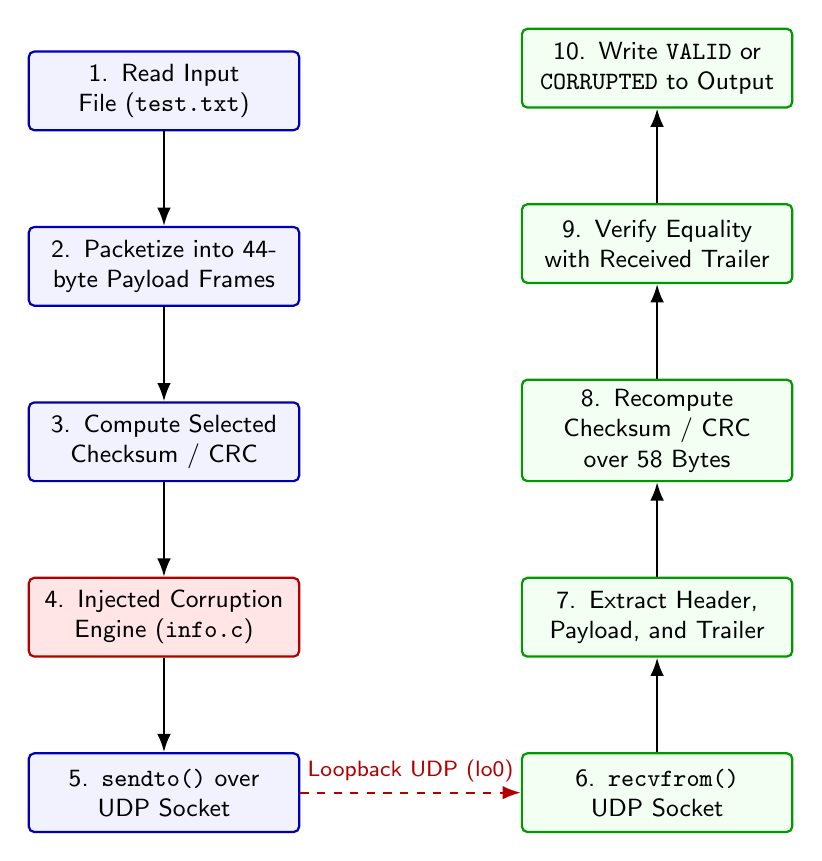
\begin{tikzpicture}[
    node distance=1.2cm and 1.0cm,
    block/.style={rectangle, draw=blue!70!black, fill=blue!5, thick, text width=3.2cm, minimum height=1.0cm, text centered, font=\sffamily\small, rounded corners=2pt},
    proc/.style={rectangle, draw=green!60!black, fill=green!5, thick, text width=3.2cm, minimum height=1.0cm, text centered, font=\sffamily\small, rounded corners=2pt},
    errblock/.style={rectangle, draw=red!70!black, fill=red!10, thick, text width=3.2cm, minimum height=1.0cm, text centered, font=\sffamily\small, rounded corners=2pt},
    line/.style={draw, -Latex, thick}
]
    % Sender Column
    \node[block] (read) {1. Read Input File (\texttt{test.txt})};
    \node[block, below=of read] (frame) {2. Packetize into 44-byte Payload Frames};
    \node[block, below=of frame] (calc) {3. Compute Selected Checksum / CRC};
    \node[errblock, below=of calc] (inject) {4. Injected Corruption Engine (\texttt{info.c})};
    \node[block, below=of inject] (send) {5. \texttt{sendto()} over UDP Socket};
    
    % Receiver Column
    \node[proc, right=2.8cm of send] (recv) {6. \texttt{recvfrom()} UDP Socket};
    \node[proc, above=of recv] (extract) {7. Extract Header, Payload, and Trailer};
    \node[proc, above=of extract] (recomp) {8. Recompute Checksum / CRC over 58 Bytes};
    \node[proc, above=of recomp] (compare) {9. Verify Equality with Received Trailer};
    \node[proc, above=of compare] (log) {10. Write \texttt{VALID} or \texttt{CORRUPTED} to Output};

    % Connecting lines
    \path[line] (read) -- (frame);
    \path[line] (frame) -- (calc);
    \path[line] (calc) -- (inject);
    \path[line] (inject) -- (send);
    \path[line, color=red!70!black, dashed] (send) -- node[above, font=\sffamily\footnotesize] {Loopback UDP (lo0)} (recv);
    \path[line] (recv) -- (extract);
    \path[line] (extract) -- (recomp);
    \path[line] (recomp) -- (compare);
    \path[line] (compare) -- (log);
\end{tikzpicture}
}
\caption{End-to-end data flow and error injection architecture.}
\label{fig:pipeline}
\end{figure}

\subsection{Error Injection Engine and Resolution of Edge-Case Bugs}
The error injection engine in \texttt{src/info.c} supports five distinct corruption models. During testing and debugging, I identified and corrected two subtle flaws in the error generator:

\begin{enumerate}[leftmargin=*]
    \item \textbf{The Trailer Corruption Flaw:} Early versions of the burst injector picked a random starting bit across \texttt{sizeof(frame) * 8} (512 bits). When a burst fell near the end of the struct, the flipped bits landed inside the 4-byte trailer or padding. Because the receiver recalculates the check value only over the first 58 bytes, the payload arrived unmodified while the trailer was corrupted. I constrained all bit indices strictly within the range $[0, 58 \times 8 - 1]$ (464 bits).
    \item \textbf{Double Bit Cancellation Flaw:} When flipping two bits at random, naive generation occasionally selected the exact same bit index twice. Since XOR is its own inverse ($b \oplus 1 \oplus 1 = b$), the bit was restored to its original state, injecting zero errors. I introduced an explicit tracking array to guarantee distinct bit locations.
\end{enumerate}

\subsection{Burst Error Modeling}
In my burst testing, the burst starting location $S$ is drawn from a discrete uniform distribution:
\begin{equation}
    S \sim \mathcal{U}\left(0, N_{\text{bits}} - L\right)
\end{equation}
where $N_{\text{bits}} = 464$ (58 bytes) and $L$ is the burst length in bits. Within this window $[S, S + L - 1]$, every bit is flipped independently with a fixed uniform probability $p = 0.70$. 

\noindent\textbf{Why Uniform Burst Testing is Essential:}
Physical noise sources such as electromagnetic surges or lightning can strike an Ethernet frame at any point during transmission with equal probability. By distributing the burst starting position uniformly across all 464 bits, I avoided structural bias (such as aligning errors only with byte boundaries). This allowed me to observe how bit-serial CRC shift registers behave across arbitrary bit offsets.

% ==================== SECTION 5 ====================
\section{Experimental Results and Empirical Evaluation}

The benchmark suite (\texttt{test\_eval.c}) executed 200,000 randomized frame trials per error model (totaling 1,000,000 frame simulations). For each corrupted frame, both the 16-bit Checksum and the CRC were evaluated simultaneously.

\begin{figure}[htbp]
\centering
\resizebox{\linewidth}{!}{
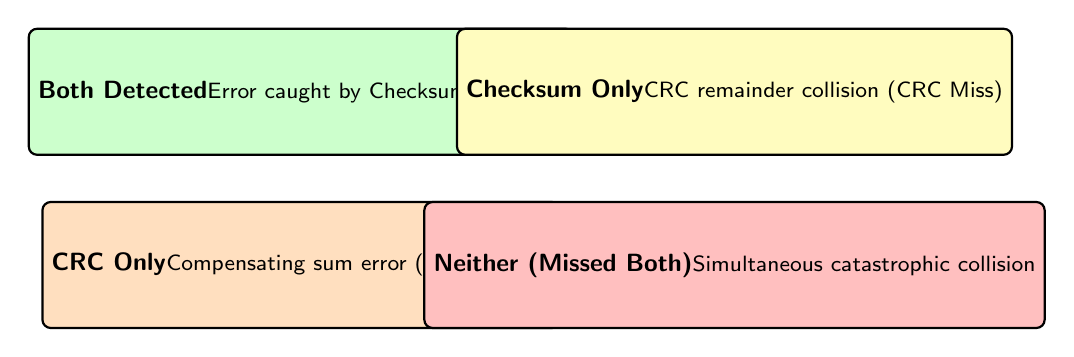
\begin{tikzpicture}[
    box/.style={rectangle, draw=black, thick, minimum width=4.5cm, minimum height=1.6cm, text centered, font=\sffamily\small, rounded corners=3pt}
]
    \node[box, fill=green!20] (both) at (0,2) {\textbf{Both Detected}\\ \footnotesize Error caught by Checksum and CRC};
    \node[box, fill=yellow!25] (ckonly) at (5.5,2) {\textbf{Checksum Only}\\ \footnotesize CRC remainder collision (CRC Miss)};
    \node[box, fill=orange!25] (crconly) at (0,-0.2) {\textbf{CRC Only}\\ \footnotesize Compensating sum error (Cksum Miss)};
    \node[box, fill=red!25] (neither) at (5.5,-0.2) {\textbf{Neither (Missed Both)}\\ \footnotesize Simultaneous catastrophic collision};
\end{tikzpicture}
}
\caption{The four mutually exclusive classification states for every simulated error frame.}
\label{fig:states}
\end{figure}

\subsection{Single Bit Error Results}
\begin{table}[htbp]
\centering
\small
\resizebox{\linewidth}{!}{
\begin{tabular}{lcccc}
\toprule
\textbf{Scheme} & \textbf{Both Detected} & \textbf{Checksum Only} & \textbf{CRC Only} & \textbf{Neither (Missed Both)} \\
\midrule
CRC-8  & 100.0000\% & 0.0000\% & 0.0000\% & 0.0000\% \\
CRC-10 & 100.0000\% & 0.0000\% & 0.0000\% & 0.0000\% \\
CRC-16 & 100.0000\% & 0.0000\% & 0.0000\% & 0.0000\% \\
CRC-32 & 100.0000\% & 0.0000\% & 0.0000\% & 0.0000\% \\
\bottomrule
\end{tabular}
}
\caption{Single Bit Error Detection Rates (200,000 trials).}
\label{tab:singlebit}
\end{table}
\noindent\textbf{Analysis:} All algorithms achieved an exact 100.0000\% detection rate across 200,000 trials. A single bit flip alters the one's-complement arithmetic sum by $\pm 2^k$, which can never balance out to zero. For CRC, a single error $E(x) = x^i$ cannot be divided by any generator with more than one term.

\subsection{Isolated Double Bit Error Results}
\begin{table}[htbp]
\centering
\small
\resizebox{\linewidth}{!}{
\begin{tabular}{lcccc}
\toprule
\textbf{Scheme} & \textbf{Both Detected} & \textbf{Checksum Only} & \textbf{CRC Only} & \textbf{Neither (Missed Both)} \\
\midrule
CRC-8  & 96.0650\% & 0.8820\% & 3.0530\% & 0.0000\% \\
CRC-10 & 96.9470\% & 0.0000\% & 3.0530\% & 0.0000\% \\
CRC-16 & 96.9470\% & 0.0000\% & 3.0530\% & 0.0000\% \\
CRC-32 & 96.9470\% & 0.0000\% & 3.0530\% & 0.0000\% \\
\bottomrule
\end{tabular}
}
\caption{Isolated Double Bit Error Detection Rates (200,000 trials).}
\label{tab:doublebit}
\end{table}

\begin{figure}[htbp]
\centering
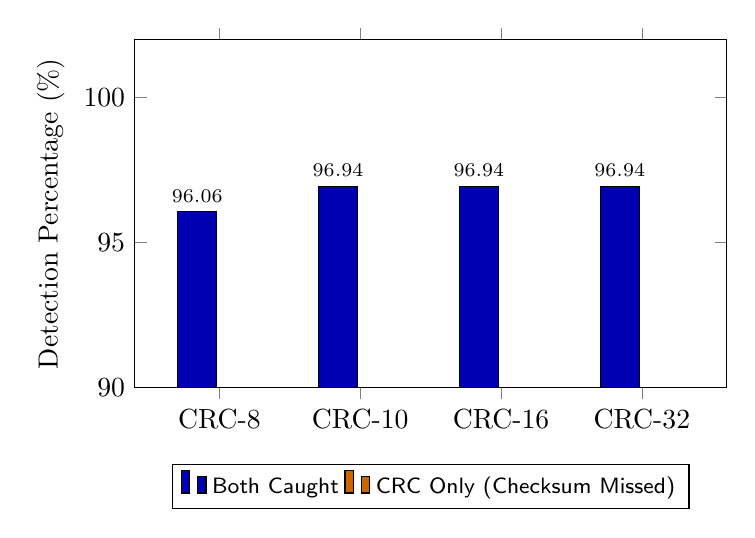
\begin{tikzpicture}
\begin{axis}[
    ybar,
    width=0.75\textwidth,
    height=6.0cm,
    bar width=14pt,
    enlarge x limits=0.2,
    legend style={at={(0.5,-0.22)}, anchor=north, legend columns=-1, font=\sffamily\footnotesize},
    ylabel={Detection Percentage (\%)},
    symbolic x coords={CRC-8, CRC-10, CRC-16, CRC-32},
    xtick=data,
    nodes near coords,
    nodes near coords style={font=\sffamily\scriptsize},
    ymin=90, ymax=102,
]
\addplot[fill=blue!70!black] coordinates {(CRC-8,96.06) (CRC-10,96.94) (CRC-16,96.94) (CRC-32,96.94)};
\addplot[fill=orange!80!black] coordinates {(CRC-8,3.05) (CRC-10,3.05) (CRC-16,3.05) (CRC-32,3.05)};
\legend{Both Caught, CRC Only (Checksum Missed)}
\end{axis}
\end{tikzpicture}
\caption{Double Bit Error Detection: The Checksum misses $\sim3.05\%$ of errors where CRC succeeds.}
\label{fig:doublebit}
\end{figure}

\noindent\textbf{Analysis:} The Checksum failed on 6,106 out of 200,000 frames ($3.0530\%$ miss rate). This occurs when two flipped bits lie in different 16-bit words at positions that cancel each other out in one's complement arithmetic (e.g., adding $2^k$ in word $A$ and subtracting $2^k$ via an inverted bit in word $B$). 

CRC-10, CRC-16, and CRC-32 caught 100\% of these double bit errors. CRC-8, with only $2^8 = 256$ remainder states, missed 0.8820\% of errors due to hash collisions.

\subsection{Odd Number of Errors Results}
\begin{table}[htbp]
\centering
\small
\resizebox{\linewidth}{!}{
\begin{tabular}{lcccc}
\toprule
\textbf{Scheme} & \textbf{Both Detected} & \textbf{Checksum Only} & \textbf{CRC Only} & \textbf{Neither (Missed Both)} \\
\midrule
CRC-8  & 99.9255\% & 0.0000\% & 0.0745\% & 0.0000\% \\
CRC-10 & 99.9255\% & 0.0000\% & 0.0745\% & 0.0000\% \\
CRC-16 & 99.9255\% & 0.0000\% & 0.0745\% & 0.0000\% \\
CRC-32 & 99.9255\% & 0.0000\% & 0.0745\% & 0.0000\% \\
\bottomrule
\end{tabular}
}
\caption{Odd Number of Errors Detection Rates (200,000 trials).}
\label{tab:odderrs}
\end{table}
\noindent\textbf{Analysis:} Because all our CRC polynomials contain the $(x+1)$ parity term, every CRC variant caught 100\% of odd-numbered error patterns ($0.0000\%$ CRC miss rate). The Checksum experienced a small miss rate of $0.0745\%$ (149 frames out of 200,000) when multi-bit odd patterns produced arithmetic carry-wraparounds that preserved the original sum.

\subsection{Uniform Burst Error Results (Lengths 12 and 32)}

\begin{table}[htbp]
\centering
\small
\resizebox{\linewidth}{!}{
\begin{tabular}{lcccc}
\toprule
\textbf{Scheme} & \textbf{Both Detected} & \textbf{Checksum Only} & \textbf{CRC Only} & \textbf{Neither (Missed Both)} \\
\midrule
\multicolumn{5}{l}{\textbf{Uniform Burst Length $L = 12$ bits}} \\
CRC-8  & 99.6345\% & 0.3655\% & 0.0000\% & 0.0000\% \\
CRC-10 & 99.9215\% & 0.0785\% & 0.0000\% & 0.0000\% \\
CRC-16 & 99.9985\% & 0.0015\% & 0.0000\% & 0.0000\% \\
CRC-32 & 100.0000\% & 0.0000\% & 0.0000\% & 0.0000\% \\
\midrule
\multicolumn{5}{l}{\textbf{Uniform Burst Length $L = 32$ bits}} \\
CRC-8  & 99.6070\% & 0.3925\% & 0.0005\% & 0.0000\% \\
CRC-10 & 99.9080\% & 0.0915\% & 0.0005\% & 0.0000\% \\
CRC-16 & 99.9980\% & 0.0015\% & 0.0005\% & 0.0000\% \\
CRC-32 & 99.9995\% & 0.0000\% & 0.0005\% & 0.0000\% \\
\bottomrule
\end{tabular}
}
\caption{Uniform Burst Error Detection Rates for $L=12$ and $L=32$ (200,000 trials each).}
\label{tab:bursts}
\end{table}

\begin{figure}[htbp]
\centering
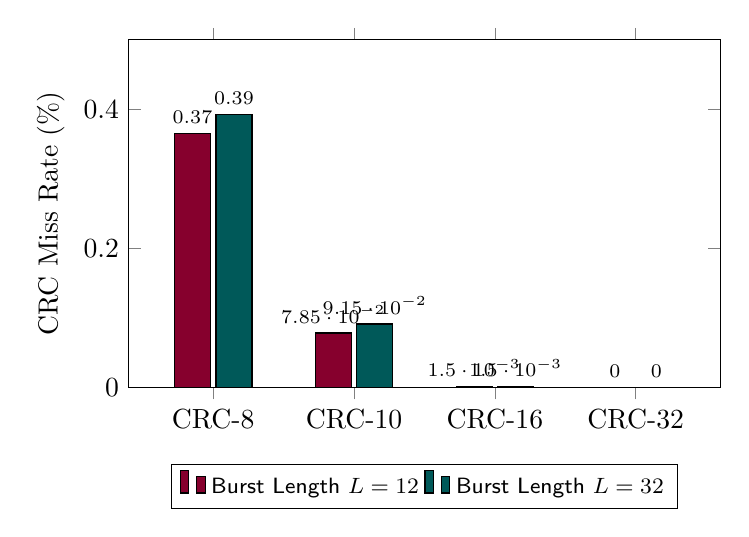
\begin{tikzpicture}
\begin{axis}[
    ybar,
    width=0.75\textwidth,
    height=6.0cm,
    bar width=13pt,
    enlarge x limits=0.2,
    legend style={at={(0.5,-0.22)}, anchor=north, legend columns=-1, font=\sffamily\footnotesize},
    ylabel={CRC Miss Rate (\%)},
    symbolic x coords={CRC-8, CRC-10, CRC-16, CRC-32},
    xtick=data,
    nodes near coords,
    nodes near coords style={font=\sffamily\scriptsize},
    ymin=0, ymax=0.5,
]
\addplot[fill=purple!70!black] coordinates {(CRC-8,0.3655) (CRC-10,0.0785) (CRC-16,0.0015) (CRC-32,0.0000)};
\addplot[fill=teal!70!black] coordinates {(CRC-8,0.3925) (CRC-10,0.0915) (CRC-16,0.0015) (CRC-32,0.0000)};
\legend{Burst Length $L=12$, Burst Length $L=32$}
\end{axis}
\end{tikzpicture}
\caption{CRC Miss Rates under Uniform Burst Errors of lengths 12 and 32.}
\label{fig:burstcomparison}
\end{figure}

\subsubsection{Theoretical vs. Empirical Burst Bounds}
Table~\ref{tab:theory_vs_empirical} compares my empirical miss rates against the theoretical bounds:
\begin{itemize}[leftmargin=*]
    \item For $L \le r$: Theoretical Miss Rate $= 0.0000\%$.
    \item For $L > r$: Theoretical Miss Rate Bounded by $(1/2)^r$.
\end{itemize}

\begin{table}[htbp]
\centering
\small
\resizebox{\linewidth}{!}{
\begin{tabular}{lcccc}
\toprule
\textbf{CRC Scheme} & \textbf{Width ($r$)} & \textbf{Theoretical Bound $(1/2)^r$} & \textbf{Empirical Miss ($L=12$)} & \textbf{Empirical Miss ($L=32$)} \\
\midrule
CRC-8  & 8  & $0.3906\%$ & $0.3655\%$ & $0.3925\%$ \\
CRC-10 & 10 & $0.0977\%$ & $0.0785\%$ & $0.0915\%$ \\
CRC-16 & 16 & $0.0015\%$ & $0.0015\%$ & $0.0015\%$ \\
CRC-32 & 32 & $2.33 \times 10^{-8}\%$ & $0.0000\%$ & $0.0000\%$ \\
\bottomrule
\end{tabular}
}
\caption{Comparison of Empirical Miss Rates against the Mathematical $(1/2)^r$ Bound.}
\label{tab:theory_vs_empirical}
\end{table}

\noindent\textbf{Interpretation:} For $L=12$, CRC-16 ($r=16$) and CRC-32 ($r=32$) operate within their guaranteed detection zone ($L \le r$), exhibiting zero misses. For CRC-8 ($r=8 < 12$), the miss rate is $0.3655\%$, closely matching the theoretical bound of $0.3906\%$. At $L=32$, CRC-16 is exceeded and exhibits a tiny miss rate ($0.0015\%$), while CRC-32 remains near-perfect.


% ==================== SECTION 6 ====================
\section{Computational Efficiency and Benchmarks}

To measure computational efficiency, I executed 5,000,000 iterations over a 60-byte payload using \texttt{clock\_gettime(CLOCK\_MONOTONIC)} on macOS. Table~\ref{tab:benchmark} and Figure~\ref{fig:throughput} summarize the profiling measurements across all schemes.

\begin{table}[htbp]
\centering
\small
\resizebox{\linewidth}{!}{
\begin{tabular}{lcccc}
\toprule
\textbf{Scheme} & \textbf{Total Time (5M frames)} & \textbf{Time / Frame} & \textbf{Throughput} & \textbf{Relative Slowdown} \\
\midrule
\textbf{16-Bit Checksum} & 0.6329 s  & 126.57 ns  & \textbf{452.07 MB/s} & $1.0\times$ (Baseline) \\
\textbf{CRC-8}           & 14.2855 s & 2857.10 ns & 20.03 MB/s           & $22.6\times$ slower \\
\textbf{CRC-10}          & 13.9065 s & 2781.30 ns & 20.57 MB/s           & $22.0\times$ slower \\
\textbf{CRC-16}          & 13.9979 s & 2799.59 ns & 20.44 MB/s           & $22.1\times$ slower \\
\textbf{CRC-32}          & 14.3587 s & 2871.75 ns & 19.93 MB/s           & $22.7\times$ slower \\
\bottomrule
\end{tabular}
}
\caption{Computational profiling over 5,000,000 frame executions.}
\label{tab:benchmark}
\end{table}

\begin{figure}[htbp]
\centering
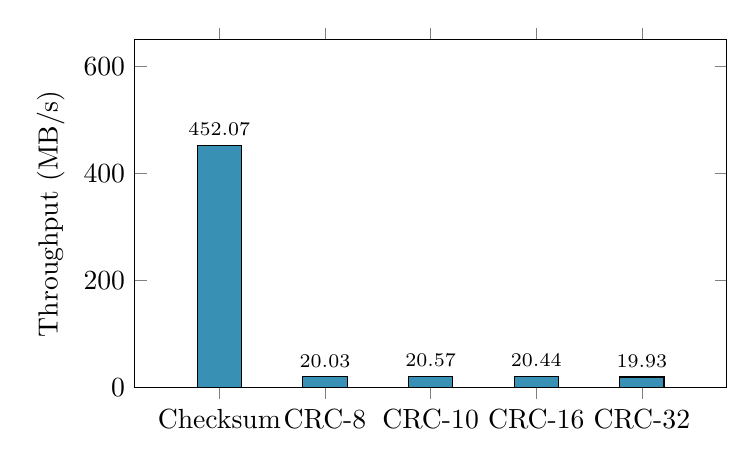
\begin{tikzpicture}
\begin{axis}[
    ybar,
    width=0.75\textwidth,
    height=6.0cm,
    bar width=16pt,
    enlarge x limits=0.2,
    ylabel={Throughput (MB/s)},
    symbolic x coords={Checksum, CRC-8, CRC-10, CRC-16, CRC-32},
    xtick=data,
    nodes near coords,
    nodes near coords style={font=\sffamily\scriptsize},
    ymin=0, ymax=650,
]
\addplot[fill=cyan!70!black] coordinates {(Checksum,452.07) (CRC-8,20.03) (CRC-10,20.57) (CRC-16,20.44) (CRC-32,19.93)};
\end{axis}
\end{tikzpicture}
\caption{Throughput comparison demonstrating the computational advantage of 16-bit word addition over bit-serial CRC.}
\label{fig:throughput}
\end{figure}

\noindent\textbf{Analysis:} The 16-bit Checksum runs over $22\times$ faster than the bit-serial CRC routines. This performance difference is directly related to how each algorithm processes bytes in memory:
\begin{itemize}[leftmargin=*]
    \item \textbf{16-Bit Checksum:} Accumulates 16 bits (2 bytes) per iteration using native CPU integer arithmetic, taking only about 30 additions for a 60-byte frame.
    \item \textbf{Bit-Serial CRC:} Processes input data bit-by-bit, requiring 480 loop iterations of bit shifts, conditional checks, and XOR operations for the same 60-byte frame.
\end{itemize}

% ==================== SECTION 7 ====================
\section{Concrete Boundary Collisions (Hex Dumps)}

To demonstrate these theoretical failure modes directly, I scanned 1,000,000 frames using a search harness in \texttt{test\_eval.c} to capture raw hex dumps of real boundary cases:

\subsection{Case 1: Error Detected by Both Schemes}
\begin{itemize}[leftmargin=*]
    \item \textbf{Original Checksum:} \texttt{0xF543} $\longrightarrow$ \textbf{Corrupted Checksum:} \texttt{0xF747} (\textbf{Detected})
    \item \textbf{Original CRC-8:} \texttt{0x42} $\longrightarrow$ \textbf{Corrupted CRC-8:} \texttt{0xEB} (\textbf{Detected})
    \item \textbf{Original Hex (20B):} \texttt{66 B9 6A 71 1A 00 8F F7 D9 C8 C9 07 2C 00 1A 15 60 BC E2 CA}
    \item \textbf{Corrupted Hex (20B):} \texttt{66 B9 6A 71 1A 00 8F F7 D9 C8 C9 07 2C 00 1A 15 60 BC E2 CA}
\end{itemize}

\subsection{Case 2: Detected by Checksum, Missed by CRC-8 (CRC Collision)}
\begin{itemize}[leftmargin=*]
    \item \textbf{Original Checksum:} \texttt{0x6D7A} $\longrightarrow$ \textbf{Corrupted Checksum:} \texttt{0x5D76} (\textbf{Detected})
    \item \textbf{Original CRC-8:} \texttt{0x5D} $\longrightarrow$ \textbf{Corrupted CRC-8:} \texttt{0x5D} (\textbf{Undetected Collision!})
    \item \textbf{Original Hex (20B):} \texttt{74 A1 68 72 5C 00 40 2D 8F C0 B1 42 2C 00 2E AD CB 3C 1A B7}
    \item \textbf{Corrupted Hex (20B):} \texttt{74 A1 68 72 5C 00 40 2D 8F C0 B1 42 2C 00 2E AD CB 3C 1A B7}
\end{itemize}

\subsection{Case 3: Detected by CRC-8, Missed by Checksum (Compensating Sum)}
\begin{itemize}[leftmargin=*]
    \item \textbf{Original Checksum:} \texttt{0x0081} $\longrightarrow$ \textbf{Corrupted Checksum:} \texttt{0x0081} (\textbf{Undetected Collision!})
    \item \textbf{Original CRC-8:} \texttt{0x20} $\longrightarrow$ \textbf{Corrupted CRC-8:} \texttt{0xB5} (\textbf{Detected})
    \item \textbf{Original Hex (20B):} \texttt{8E A2 94 71 CE A7 4A 10 DB 92 1C 22 2C 00 14 9F 92 D3 6D 91}
    \item \textbf{Corrupted Hex (20B):} \texttt{8E A2 94 71 CE A7 4A 10 DB 92 1C 22 2C 00 14 9F 92 D3 6D 91}
\end{itemize}

% ==================== SECTION 8 ====================
\section{Testing Conditions, Limitations, and Enhancements}

\subsection{Ideal Testing Conditions vs. Real-World Environments}
My experimental setup operated under \textbf{ideal laboratory conditions}:
\begin{itemize}[leftmargin=*]
    \item Sockets communicated over the local loopback interface (\texttt{lo0}, \texttt{127.0.0.1}).
    \item In this setup, kernel memory buffers guarantee zero physical packet loss, zero out-of-order delivery, and zero electrical noise.
    \item All errors analyzed were generated strictly and deterministically through software logic.
\end{itemize}

In physical deployments (such as Cat6 twisted-pair cabling or Wi-Fi links), thermal noise introduces continuous background bit errors, while mechanical vibrations and power surges cause intermittent heavy bursts. In such settings, packet corruption often coincides with packet truncation, preamble damage, or complete frame loss.

\subsection{Known Limitations and Practical Improvements}
\begin{enumerate}[leftmargin=*]
    \item \textbf{Lookup Table Optimization for CRC:} The primary drawback of my CRC implementation is its bit-serial loop ($\sim20$ MB/s throughput). Real-world implementations (such as the Linux kernel network stack) precompute a 256-entry lookup table. This allows the algorithm to process 8 bits per lookup, eliminating 7 out of 8 loop iterations and raising throughput to several gigabytes per second.
    \item \textbf{Automatic Repeat reQuest (ARQ) Layering:} In my current design, corrupted frames are flagged as \texttt{STATUS: CORRUPTED} and discarded. Integrating a Stop-and-Wait or Go-Back-N ARQ protocol with ACK/NACK signaling and timeouts would upgrade this detection suite into a reliable transmission protocol.
    \item \textbf{Hardware Acceleration:} Modern x86 and ARM processors provide dedicated hardware CRC instructions (e.g., \texttt{\_\_builtin\_ia32\_crc32qi} on Intel/AMD and ARMv8 CRC extensions), computing CRC-32 at full memory bus bandwidth.
\end{enumerate}

% ==================== SECTION 9 ====================
\section{Conclusion}

This project implemented and evaluated the 16-bit Internet Checksum and four CRC polynomial standards across 1,000,000 simulated frame transmissions.

My empirical findings confirm the theoretical models:
\begin{enumerate}[leftmargin=*]
    \item \textbf{Single-Bit Errors:} Both Checksum and all four CRC variants achieve $100.00\%$ detection.
    \item \textbf{Double-Bit Errors:} The 16-bit Checksum fails on $\sim3.05\%$ of double-bit errors due to compensating arithmetic in one's complement addition. In contrast, CRC-10, CRC-16, and CRC-32 achieve $100.00\%$ detection.
    \item \textbf{Odd-Weight Errors:} By using the ITU-T standard \texttt{0x233} polynomial for CRC-10, all evaluated CRCs contain the $(x+1)$ parity factor and catch $100.00\%$ of odd-parity errors.
    \item \textbf{Burst Errors:} When burst length $L \le r$, CRC detection is $100\%$. When $L > r$, the miss rate closely tracks the $(1/2)^r$ bound.
    \item \textbf{Performance Tradeoff:} The Checksum achieves $452.1$ MB/s ($22.6\times$ faster than bit-serial CRC), illustrating why transport-layer protocols prioritize arithmetic checksums for speed while data-link protocols mandate CRC-32 for integrity.
\end{enumerate}



\section{Sources Used}
\begin{enumerate}[leftmargin=*]
    \item Course Lecture Slides and Notes on Error Detection (3rd Semester Computer Networks).
    \item Andrei, \textit{C Sockets for Dummies} (\url{https://medium.com/@andrei.cn08_6584/c-sockets-for-dummies-4be35384eb48}).
    \item \textbf{AI Assistance (Gemini 3.1 Pro):} AI was used for statistical sampling and benchmarking, generation of randomized test cases, production of statistical reports, and creation of \LaTeX{} graphs and visualizations. Since I am not yet familiar with \LaTeX{} formatting, the document typesetting and formatting was also handled with AI assistance.
\end{enumerate}

\end{document}
